% compile with XeLaTeX
\documentclass[dvipsnames,mathserif]{beamer}
\setbeamertemplate{footline}[frame number]
\setbeamercolor{footline}{fg=black}
\setbeamerfont{footline}{series=\bfseries}
\usepackage{tikz}
\usepackage{adjustbox}
\usepackage{subcaption}
\usepackage{graphicx}
\usepackage{enumitem}
\usepackage{fancyvrb}
\usepackage{colortbl}
\usepackage{booktabs}% http://ctan.org/pkg/booktabs

%\usetheme{Frankfurt}%1
\usetheme{Darmstadt}%1

% for RTL liste
\makeatletter
\newcommand{\RTListe}{\raggedleft\rightskip\leftm}
\newcommand{\leftm}{\@totalleftmargin}
\makeatother

% RTL frame title
\setbeamertemplate{frametitle}
{\vspace*{-1mm}
  \nointerlineskip
  \begin{beamercolorbox}[sep=0.3cm,ht=2.2em,wd=\paperwidth]{frametitle}
    \vbox{}\vskip-2ex%
    \strut\hskip1ex\insertframetitle\strut
    \vskip-0.8ex%
  \end{beamercolorbox}
}
% align subsection in toc
\makeatletter
\setbeamertemplate{subsection in toc}
{\leavevmode\rightskip=5ex%
  \llap{\raise0.1ex\beamer@usesphere{subsection number projected}{bigsphere}\kern1ex}%
  \inserttocsubsection\par%
}
\makeatother

% RTL triangle for itemize
\setbeamertemplate{itemize item}{\scriptsize\raise1.25pt\hbox{\donotcoloroutermaths$\blacktriangleleft$}}

%\setbeamertemplate{itemize item}{\rule{4pt}{4pt}}

\defbeamertemplate{enumerate item}{square2}
{\LR{
    %
    \hbox{%
      \usebeamerfont*{item projected}%
      \usebeamercolor[bg]{item projected}%
      \vrule width2.25ex height1.85ex depth.4ex%
      \hskip-2.25ex%
      \hbox to2.25ex{%
        \hfil%
        {\color{fg}\insertenumlabel}%
      \hfil}%
    }%
}}

\setbeamertemplate{enumerate item}[square2]
\setbeamertemplate{navigation symbols}{}


\titlegraphic {
  \begin{tikzpicture}[overlay,remember picture, opacity=0.1,]
    \node[] at (0, 2.9){
        \includegraphics[width=0.63\textwidth]{udglogo.png}
  };\end{tikzpicture}}
  \setbeamertemplate{caption}[numbered]
  \begin{document}

  \rightskip\rightmargin
  \title{A Platform for Classifying Melanoma}
  \author{ \Large \textbf{Wilber Eduardo Bermeo Quito} }
  \institute{\large\textbf{Master in Data Science}\\
    ---------\\
    Higher Polytechnic School\\
    ---------\\
  University of Girona}
  \footnotesize{\date{\today }


    \begin{frame}
      \maketitle
    \end{frame}

    \begin{frame}{Summery}
      \footnotesize \tableofcontents

    \end{frame}

    \section{Introduction}


    \begin{frame}
      \frametitle{Introduction}
    \end{frame}


    \begin{frame}
      \large Motivations
      \vspace{0.25cm}

      \footnotesize
      \begin{itemize}
        \item Enhance AI\footnote{Artificial Intelligence.} knowledge.
        \item Automation as way to democratize access to research and AI solutions.
        \item CAD\footnote{Computer-Aided Diagnosis.} system are promising path
          towards medical automation.
      \end{itemize}
    \end{frame}


    \begin{frame}
      \large Objectives
      \vspace{0.25cm}

      \footnotesize
      \begin{itemize}
        \item Gain expertise in deep learning theory and its real-world
          applications.
        \item Explore and study the optimal approach for utilizing the distribution
          of dermoscopy images from the dataset during the training process.
        \item Propose and train deep learning models using transfer learning on ISIC\footnote{Skin Imaging Collaboration.}
          Challenge melanoma images.
        \item Create an easy deployment CAD infrastructure running in Docker,
          with the trained models, a user-friendly web UI\footnote{User
          Interface.} and a HTTP API\footnote{Application Programming Interface.}.
      \end{itemize}


    \end{frame}

    \section{Domain}

    \begin{frame}
      \frametitle{Domain}
    \end{frame}

    \begin{frame}
      \begin{center}
        \Huge Problem
      \end{center}
    \end{frame}


    \begin{frame}
      \large Detection of Melanoma Skin Cancer
      \vspace{0.25cm}

      \footnotesize
      \begin{itemize}
        \item Melanoma exhibits a high mortality rate.
        \item Dermoscopy procedures are utilized for melanoma detection.
        \item Dermoscopy images are examined by professionals to study cutaneous lesions.
        \item Several studies have shown that melanoma task classification
          using CAD systems achieve comparable or superior results to
          dermatologists.
      \end{itemize}


    \end{frame}



    \begin{frame}

    \large Metastasis
      \vspace{0.25cm}

      \footnotesize
    \begin{figure}[H] \centering
      \includegraphics[width=0.5\textwidth]{images/stage3-skin-cancer.jpg}
      \caption[Skin Cancer, Stage III]{\textit{Skin Cancer, Stage III. Illustration by
    Terese Winslow}} {\label{fig:stage3-skin-canceer}} \end{figure}

    \end{frame}

    \begin{frame}
      \begin{center}
        \Huge Solution
      \end{center}
    \end{frame}


    \begin{frame}

      \large CAD Training and Deployment Pipeline
      \vspace{0.25cm}

      \begin{figure}[H]
        %\begin{adjustbox}{width=\textwidth, trim={0.2cm 0pt 1.5cm 0pt}, clip}
        \centering
        \includegraphics[width=0.7\textwidth]{images/Pipeline.drawio.png}
        %\end{adjustbox}
        \caption[CAD Infrastructure Pipeline]{\textit{CAD Infrastructure Pipeline.}}
        {\label{fig:cad-infrastructure-training-system}}
      \end{figure}

    \end{frame}

    \begin{frame}
      \large Micro-Service Architecture to Infer Images
      \vspace{0.25cm}

      \begin{figure}[H]
        \centering
        \includegraphics[width=0.65\textwidth]{images/BackgroundTask.drawio.png}
        \caption[Inferring Images Through the Background Task Mechanism]{\textit{Inferring Images Through the Background Task Mechanism.  }}
        {\label{fig:backgrond-task}}
      \end{figure}

    \end{frame}





    \section{Concerns}


    \begin{frame}
      \frametitle{Concerns}
    \end{frame}

    \begin{frame}
      \large Ethical Concern
      \vspace{0.25cm}

      \footnotesize
      \begin{itemize}
        \item The solution employs "black box" models, lacking explain-ability.
        \item The thesis presents a CAD tool designed to aid human decision-making
          rather than being an autonomous decision-making system.
      \end{itemize}
    \end{frame}

    \begin{frame}

      \large Regulatory Framework
      \vspace{0.25cm}

      \footnotesize

      \begin{itemize}
        \item When dealing with medical images, obtaining signed consent is
          necessary for data publication.
        \item Recent research collaborations prioritize data sharing through
          de-identification methods to tackle these challenges.
        \item The thesis made use of the ISIC Archive database, which serves as
          a publicly accessible resource.
      \end{itemize}


    \end{frame}



    \section{Data}

    \begin{frame}
      \frametitle{Data}
    \end{frame}

    \begin{frame}

      \large Origin Data Decription
      \vspace{0.25cm}

      \footnotesize

      \begin{itemize}
        \item The data originates from the ISIC Archive.
        \item It includes images from the years 2019 and 2020.
        \item The images are available in three different resolutions: 512x512,
          768x768, and 1024x1024 pixels.
        \item The dataset contains more than eight distinct classes.
      \end{itemize}

    \end{frame}


    \begin{frame}

      \large Used Data Decription
      \vspace{0.25cm}

      \footnotesize

      \begin{itemize}
        \item Resolution selected: 512x512 pixels.
        \item The used dataset comprises 31,265 distinct image samples.
        \item Eight classes were selected to work with.
        \item Imbalanced dataset.
      \end{itemize}

    \end{frame}

    \begin{frame}

      \large Classes Distribution in the Dataset
          \vspace{0.25cm}

      \begin{figure}[H]
        \centering
        \includegraphics[width=0.7\textwidth]{images/hole-dataset-diagnosis.png}
        \caption[Data Distribution]{\textit{Data Distribution. }}
        {\label{fig:hole-dataset-distribution}}
      \end{figure}

    \end{frame}

    \begin{frame}

      \large  Train, Validation and Test Sets
      \vspace{0.25cm}

      \footnotesize

      \begin{itemize}
        \item The dataset was stratified to ensure an equal distribution of classes in each subset.
        \item The training set was created using 80\% of the dataset, the validation set using 10\%, and the test set using the remaining 10\%.
      \end{itemize}


      \begin{figure}[H]
        \centering
        \begin{adjustbox}{width=0.5\textwidth, trim={0cm 0.5cm 0cm 0.5cm}, clip}
          \includegraphics[width=\textwidth]{images/train-test-validation-sets.png}
        \end{adjustbox}
        \caption[Holdout Set Scheme]{\textit{Holdout Set Scheme. Illustration by Qualcomm}}
        {\label{fig:holdout-test-scheme}}
      \end{figure}

    \end{frame}

    \begin{frame}

      \large Data Augmentation
      \vspace{0.25cm}

      \footnotesize

      The train dataset (Figure \ref{fig:sample-of-datasets}),

      \begin{figure}[H]
        \centering
        \includegraphics[width=0.6\textwidth]{images/random-sample-of-isic.png}
        \caption[Random Sample of Images]{\footnotesize{\textit{Random Sample of Images.}}}
        {\label{fig:sample-of-datasets}}
      \end{figure}

      Is mapped into an augmented train dataset (Figure \ref{fig:aug-sample-of-datasets}).

      \begin{figure}[H]
        \centering
        \includegraphics[width=0.6\textwidth]{images/random-sample-of-isic-augmented.png}
        \caption[Augmented Random Sample of Images]{\footnotesize{\textit{Augmented Random Sample of Images.}}}
        {\label{fig:aug-sample-of-datasets}}
      \end{figure}

    \end{frame}



%
    \section{Modeling}

    \begin{frame}
      \frametitle{Modeling}
    \end{frame}

    \begin{frame}

      \large General Modeling Information
          \vspace{0.25cm}

      \footnotesize

      \begin{itemize}
        \item Eight trained models with different ML thecniques.
        \item Used the ResNet18 pre-trained weights.
        \item SGD as optimizer.
        \item Cross-entropy as loss function.
        \item Model training performance were evaluated with AUC metric.
      \end{itemize}

    \end{frame}

    \begin{frame}


  \begin{table}

    \centering
    \begin{adjustbox}{width=\textwidth}
    \begin{tabular}{lcccccccc}
      \toprule
      & \textbf{M0} & \textbf{M1} & \textbf{M2} & \textbf{M3} & \textbf{M4} & \textbf{M5} & \textbf{M6} & \textbf{M7} \\
      \midrule
      Model Architecture & R18M & R18M & R18M & R18M & R18DM & R18DM & R18DM & R18DM \\
      Epochs & 20 & 20 & 20 & 20 & 40 & 40 & 40 & 40 \\
      Batch Size & 400 & 400 & 400 & 400 & 1024 & 1024 & 1024 & 1024 \\
      Scheduler & & SLR & CALR & CAWR &  & SLR & CALR & CAWR  \\
      Data Augmentation & No & No & No & No  & Yes & Yes & Yes & Yes \\
      Dropout Regularization & No & No & No & No  & Yes & Yes & Yes & Yes \\
      GPU & TT4 & TT4 & TT4 & TT4 & NA100 & NA100 & NA100 & NA100 \\
      Training Time & 1h 45m & 1h 22m & 1h 43m & 1h 38m & 1d 7h 30m & 1d 7h 4m & 1d 7h 1m & 1d 12h 55m \\ \bottomrule
    \end{tabular}
  \end{adjustbox}
    \caption[Training Information For Each Model.]
    {\textit{\footnotesize{Training Information For Each Model. Empty spaces represent non-use of that feature.}}}
    {\label{table:trained-models-information}}
  \end{table}

    \end{frame}


    \begin{frame}

  \begin{table}
    \centering
    \begin{adjustbox}{width=\textwidth}
    \begin{tabular}{lccccccccc}
      \toprule
      & \textbf{Train AUC} & \textbf{Val AUC} & \textbf{Test AUC} & \textbf{Train Recall} & \textbf{Val Recall} & \textbf{Test Recall} & \textbf{Train Acc} & \textbf{Val Acc} & \textbf{Test Acc} \\
      \midrule
      M0 & 0.952 & 0.903 & 0.892 & 0.756 & 0.676 & 0.652 & 0.835 & 0.778 & 0.772 \\
      M1 $\star$ & 0.947 & 0.900 & 0.892 & 0.695 & 0.633 & 0.599 & 0.829 & 0.779 & 0.771 \\
      M2 $\ast$ & 0.933 & 0.895 & 0.885 & 0.658 & 0.609 & 0.582 & 0.808 & 0.765 & 0.762 \\
      M3 $\bullet$ & 0.935 & 0.896 & 0.886 & 0.663 & 0.605 & 0.589 & 0.811 & 0.767 & 0.764 \\
      \midrule
      \cellcolor{gray!50}M4 & \cellcolor{gray!50}0.886 & \cellcolor{gray!50}0.877 & \cellcolor{gray!50}0.858 & \cellcolor{gray!50}0.478 & \cellcolor{gray!50}0.475 & \cellcolor{gray!50}0.446 & \cellcolor{gray!50}0.757 & \cellcolor{gray!50}0.750 & \cellcolor{gray!50}0.741 \\
      \cellcolor{gray!50}M5 $\star$ & \cellcolor{gray!50}0.867 & \cellcolor{gray!50}0.861 & \cellcolor{gray!50}0.843 & \cellcolor{gray!50}0.423 & \cellcolor{gray!50}0.403 & \cellcolor{gray!50}0.395 & \cellcolor{gray!50}0.728 & \cellcolor{gray!50}0.717 &  \cellcolor{gray!50}0.715 \\
      \cellcolor{gray!50}M6 $\ast$ & \cellcolor{gray!50}0.874 & \cellcolor{gray!50}0.868 & \cellcolor{gray!50}0.848 & \cellcolor{gray!50}0.451 & \cellcolor{gray!50}0.440 & \cellcolor{gray!50}0.418 & \cellcolor{gray!50}0.738 & \cellcolor{gray!50}0.728 &  \cellcolor{gray!50}0.722 \\
      \cellcolor{gray!50}M7 $\bullet$ & \cellcolor{gray!50}0.877 & \cellcolor{gray!50}0.869 & \cellcolor{gray!50}0.849 & \cellcolor{gray!50}0.470 & \cellcolor{gray!50}0.458 & \cellcolor{gray!50}0.432 & \cellcolor{gray!50}0.742 & \cellcolor{gray!50}0.732 &  \cellcolor{gray!50}0.723 \\

      \midrule

      Mean &  94.175\% & 89.850\% & 88.875\%  & 69.300\% & 63.075\% & 60.550\% & 82.075\% & 77.225\% & 76.725\% \\
      SD   & 0.921\% & 0.370\% & 0.377\%  &  4.509\% & 3.260\% & 3.178\% & 1.327\% & 0.727\% & 0.499\% \\

      \midrule

      \cellcolor{gray!50}Mean & \cellcolor{gray!50}87.600\% & \cellcolor{gray!50}86.875\% & \cellcolor{gray!50}84.950\% & \cellcolor{gray!50}45.550\% & \cellcolor{gray!50}44.400\% & \cellcolor{gray!50}42.275\% & \cellcolor{gray!50}74.125\% & \cellcolor{gray!50}73.175\% & \cellcolor{gray!50}72.525\% \\
      \cellcolor{gray!50}SD & \cellcolor{gray!50}0.787\% & \cellcolor{gray!50}0.655\% & \cellcolor{gray!50}0.625\% & \cellcolor{gray!50}2.445\% & \cellcolor{gray!50}3.084\% & \cellcolor{gray!50}2.175\% & \cellcolor{gray!50}1.204\% & \cellcolor{gray!50}1.372\% &  \cellcolor{gray!50}1.108\% \\

      \bottomrule
    \end{tabular}
  \end{adjustbox}
    \caption[Metrics in the Datasets]
    {\textit{Metrics in the Datasets. }}
    {\label{table:resume-metrics}}
  \end{table}
    \end{frame}




    \section{Services}

    \begin{frame}

      \large API
      \vspace{0.25cm}

    \end{frame}


    \begin{frame}
      \large UI
      \vspace{0.25cm}
    \end{frame}


    \begin{frame}
      \large Containers
      \vspace{0.25cm}


      \begin{itemize}
        \item Easy to maintain.
        \item Portable.
        \item Fast to start-up.
      \end{itemize}


    \end{frame}

    \section{Results}

    \begin{frame}
      \footnotesize
      System behavior without controller
      \begin{figure}[H]
        \centering
        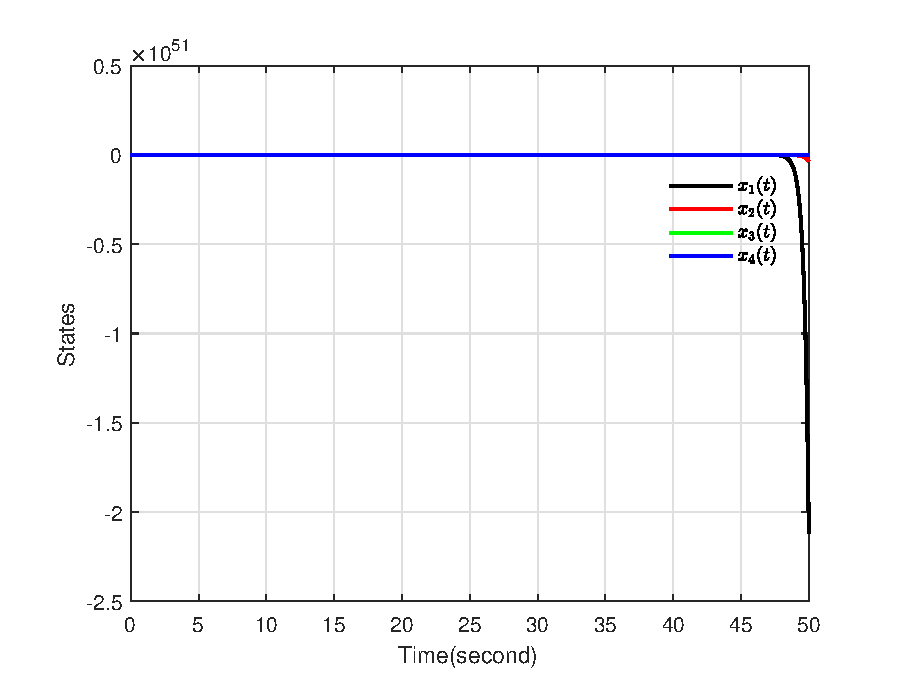
\includegraphics[width=0.75\textwidth]{x_1.eps}
        \caption{System state}
      \end{figure}
      System unstable
    \end{frame}

    \begin{frame}
      System behavior with controller

      \begin{figure}[H]
        \centering
        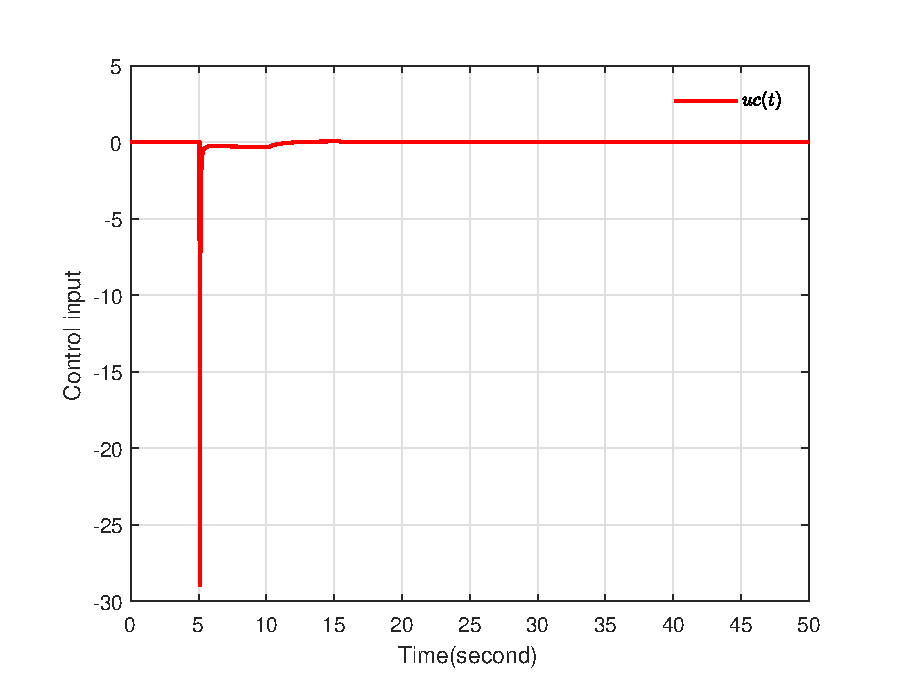
\includegraphics[width=0.75\textwidth]{kuc.eps}
        \caption{Control signal }
        \label{fig3.3}
      \end{figure}
    \end{frame}
    \begin{frame}
      System behavior with controller
      \begin{figure}[H]
        \centering
        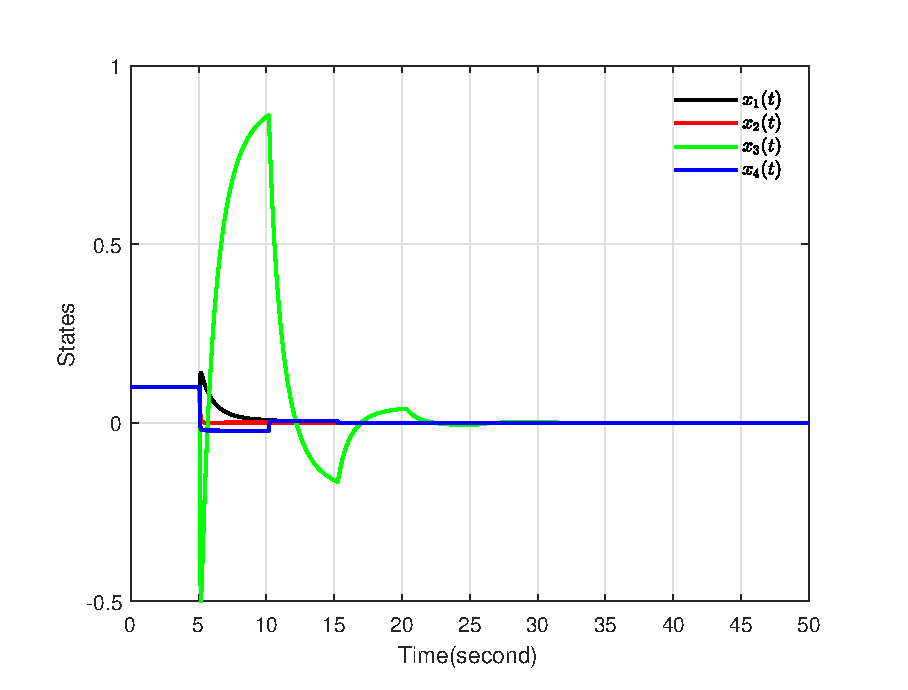
\includegraphics[width=0.75\textwidth]{kstates.eps}
        \caption{System state}
        \label{fig3.4}
      \end{figure}

      The system is stable but it needs more enhancement
    \end{frame}


    \begin{frame}
      System behavior with the proposed controller
      \begin{figure}[H]
        \centering
        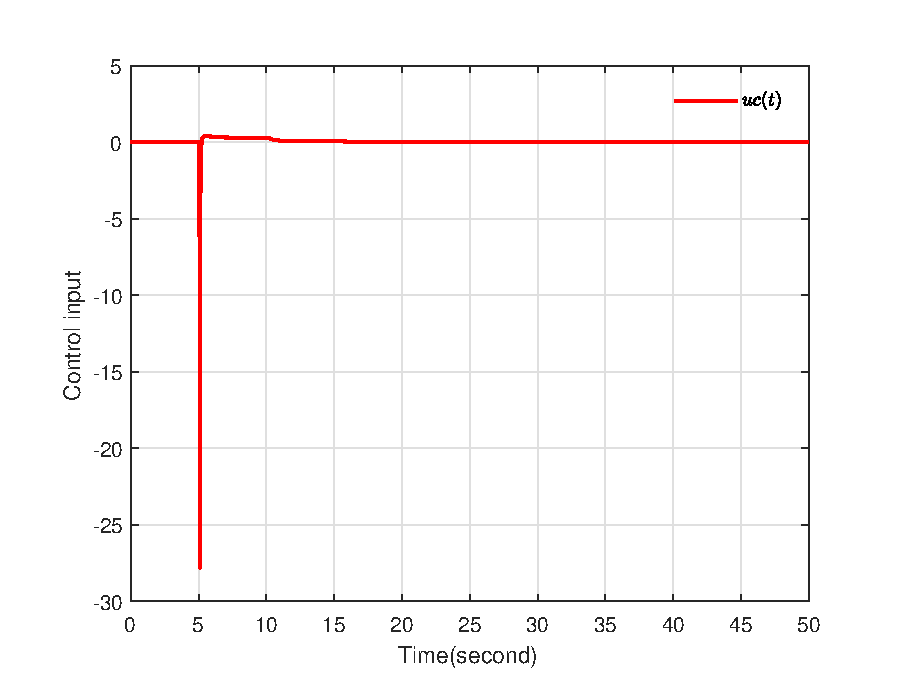
\includegraphics[width=0.75\textwidth]{2uc.eps}
        \caption{Proposed controller signal }
        \label{fig3.5}
      \end{figure}
    \end{frame}
    \begin{frame}
      System behavior with the proposed controller

      \begin{figure}[H]
        \centering
        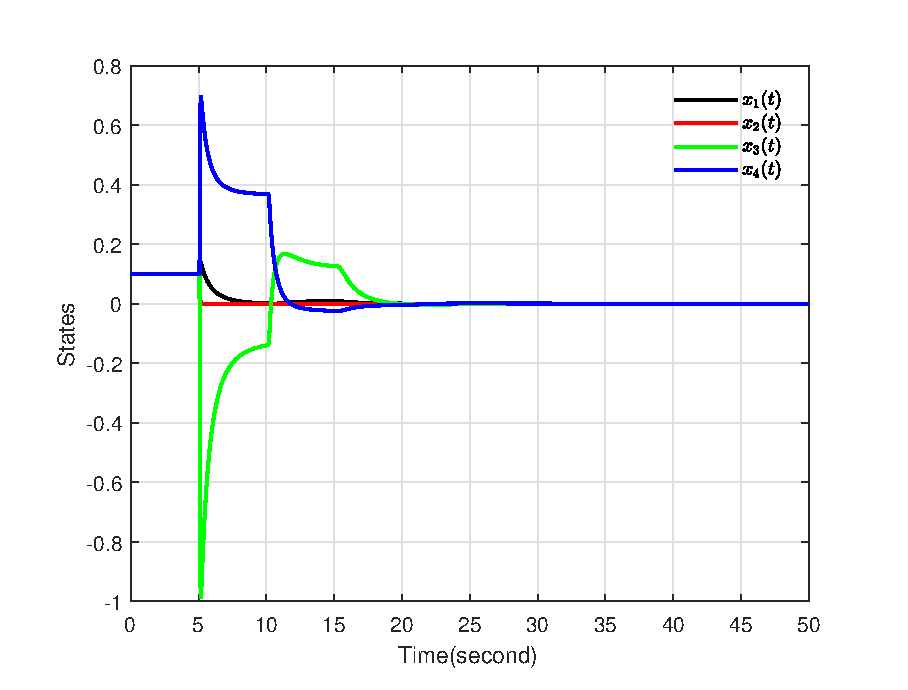
\includegraphics[width=0.75\textwidth]{2states.eps}
        \caption{System state with the proposed controller }
        \label{fig3.6}
      \end{figure}

      \textcolor{blue}{ Stability + better performance}

    \end{frame}

    \begin{frame}
      \footnotesize
      Quantification of the comparative study
      \begin{table}[h]
        \centering
        \begin{tabular}{|*{4}{c|}}
          \hline
  & Classical controller & Proposed controller & Enhancement rate \\
  \hline
          Settling time & $26$  &  $20$ & 23 \% \\
          \hline
          Pic to pic $x_3$  &$1.36$ & $1.16 $ &15 \% \\
          \hline
          $\int\limits_0^{ts}(x_3^2)dt $
                            & $2.5540$ & $0.7771$& 70 \% \\
                            \hline
          $ \int\limits_0^{ts}(u^2)dt$ & $12.8476$ & $7.1868$& 40 \% \\
          \hline
        \end{tabular}
        \caption{Quantification of the comparative study}
      \end{table}
      We remark that
      \begin{itemize}
        \item \textcolor{blue}{\textbf{Enhancement of the settling time of $23\%$}}
        \item \textcolor{blue}{\textbf{ Reduction of the control energy by $40\%$}}
        \item \textcolor{blue}{\textbf{ Overall enhancement by  $70\%$ }}
        \item \textcolor{blue}{\textbf{ Pic to pic reduction by  $15\%$}}
      \end{itemize}
    \end{frame}

    \section{Conclusion and Perspectives}
    \begin{frame}
      \footnotesize
      We conclude that:
      \begin{block}{Conclusion}
        \begin{itemize}
          \item  \textcolor{blue}{\textbf{Lyapunov method efficiency.}}
          \item \textcolor{blue}{\textbf{Proposed controller leads to better performance.}}
          \item \textcolor{blue}{\textbf{Delayed controller enhances the performance.}}
          \item \textcolor{blue}{\textbf{Proposed approach allows reduction of the control energy.}}
        \end{itemize}
      \end{block}
      As perspectives we propose:
      \begin{block}{perspectives}
        \begin{itemize}
          \item Perspective 1.
          \item Perspective 2.
          \item Perspective 3.
        \end{itemize}
      \end{block}
    \end{frame}


    \end{document}
